\documentclass[11pt]{article}
\usepackage[margin=0.7in]{geometry}
\usepackage{amsmath,amssymb}
\usepackage{enumitem}
\usepackage{tikz}
\usepackage{pgfplots}
\pgfplotsset{compat=1.18}
\usepackage{fancyhdr}
\usepackage{parskip}
\setlist[enumerate]{leftmargin=*, itemsep=6pt}
\pagestyle{fancy}
\fancyhf{}
\fancyfoot[L]{\small\textit{en}Vision\textsuperscript{\textregistered} Algebra 2}
\fancyfoot[C]{\small 3-7 Lesson Quiz, short form}
\fancyfoot[R]{\small\thepage}
\renewcommand{\headrulewidth}{0pt}
\newcommand{\choice}[1]{\tikz[baseline=-0.6ex]\node[draw, circle, inner sep=0.6pt, minimum size=3.3mm, font=\scriptsize\bfseries] {#1};\;}
\newcommand{\checkbox}{$\square$\;}
\pgfplotsset{quizgrid/.style={
  axis lines=middle, grid=both, grid style={gray!45},
  ticklabel style={font=\scriptsize, fill=white, inner sep=1pt},
  xlabel={$x$}, ylabel={$y$}, axis line style={thick}, clip=true}}

\begin{document}

\noindent\textbf{Name}\; \rule{6cm}{0.4pt} \hfill Period \rule{1.2cm}{0.4pt} \quad Date \rule{2.2cm}{0.4pt}

\vspace{4pt}\noindent\rule{\textwidth}{0.6pt}

\vspace{2pt}\noindent{\Large\textbf{3-7 \; Lesson Quiz: Transformations of Polynomial Functions}} \hfill {\small short form}

\vspace{4pt}\noindent\rule{\textwidth}{0.6pt}

\vspace{4pt}
\textbf{2.} Identify the parent function of the function $f(x)=-x^4-1$, and list the transformations from the parent function to create $f(x)$.

\vspace{2pt}
\begin{itemize}[leftmargin=1.2em, itemsep=1pt, topsep=1pt]
\item[] \choice{A} $x^4$; translate down 1 unit, reflect over the $x$-axis
\item[] \choice{B} $x^4$; reflect over the $x$-axis, translate down 1 unit
\item[] \choice{C} $x^3$; reflect over the $x$-axis, translate down 1 unit
\item[] \choice{D} $x^3$; compress the graph by a factor of $x$, translate down 1 unit
\end{itemize}

\vspace{4pt}
Explain your choice: why is the order of the two transformations in your answer the right order?

\vspace{14pt}\rule{\textwidth}{0.4pt}

\vspace{6pt}\noindent\rule{\textwidth}{0.4pt}

\vspace{4pt}
\textbf{3.} How does the graph of $g(x)=3x^3+6$ differ from the graph of its parent function $f(x)=x^3$? Select \textbf{all} the transformations.

\vspace{2pt}
\begin{itemize}[leftmargin=1.2em, itemsep=1pt, topsep=1pt]
\item[] \checkbox \textbf{A.} The leading coefficient, 3, translates the graph up 3 units.
\item[] \checkbox \textbf{B.} The leading coefficient, 6, compresses the graph vertically.
\item[] \checkbox \textbf{C.} The leading coefficient, 3, stretches the graph vertically.
\item[] \checkbox \textbf{D.} Adding 6 translates the graph up 6 units.
\item[] \checkbox \textbf{E.} Adding 6 translates the graph right 6 units.
\end{itemize}


\vspace{6pt}\noindent\rule{\textwidth}{0.4pt}

\vspace{4pt}
\begin{minipage}[t]{0.52\textwidth}
\textbf{4.} Determine the equation of the graph as it relates to either its parent cubic function or quartic function.

\vspace{4pt}
\begin{itemize}[leftmargin=1.2em, itemsep=3pt, topsep=2pt]
\item[] \choice{A} $f(x)=(x-2)^3-3$
\item[] \choice{B} $f(x)=(x-3)^4-2$
\item[] \choice{C} $f(x)=(x+3)^4+2$
\item[] \choice{D} $f(x)=(x-2)^4-3$
\end{itemize}

\vspace{6pt}
Explain your choice: how does the graph show whether the parent function is cubic or quartic?

\vspace{12pt}\rule{\linewidth}{0.4pt}
\end{minipage}\hfill
\begin{minipage}[t]{0.44\textwidth}
\vspace{-4pt}
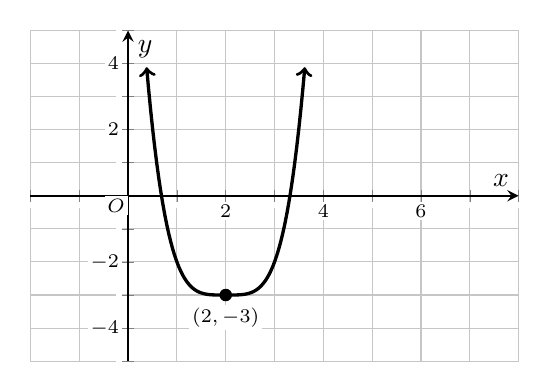
\begin{tikzpicture}
\begin{axis}[quizgrid, xmin=-2, xmax=8, ymin=-5, ymax=5,
  xtick={-2,...,8}, xticklabels={,,,,$2$,,$4$,,$6$,,},
  ytick={-5,...,5}, yticklabels={,$-4$,,$-2$,,,,$2$,,$4$,},
  x=0.62cm, y=0.42cm]
\addplot[very thick, domain=0.38:3.62, samples=80, <->] {(x-2)^4-3};
\node[font=\scriptsize, fill=white, inner sep=1pt, anchor=north east] at (axis cs:0,0) {$O$};
\node[circle, fill, inner sep=1.6pt] at (axis cs:2,-3) {};
\node[font=\scriptsize, fill=white, inner sep=1pt, anchor=north] at (axis cs:2,-3.3) {$(2,-3)$};
\end{axis}
\end{tikzpicture}
\end{minipage}

\vfill
\noindent\textbf{Scoring:} Question 2 and Question 3 are 10 points each. Question 4 is a bonus of up to 5 points. Total out of 20. {\small (Numbers match the Savvas Lesson Quiz; Questions 1 and 5 are not on this form.)}

\newpage
\noindent{\LARGE\textbf{3-7 Lesson Quiz, short form: answer key}}

\vspace{4pt}\noindent\rule{\textwidth}{0.6pt}

\begin{enumerate}
\item[2.] \textbf{B.} $-x^4-1$ is $x^4$ multiplied by $-1$ (reflection over the $x$-axis) and then $1$ subtracted (translate down 1). Translating first and then reflecting gives $-(x^4-1)=-x^4+1$, which is why A is wrong; C and D have the wrong parent (the degree is 4). Savvas item 2, DOK 2, Realize skill F63. Taught by Example 3 (stretch before the vertical translation) and rehearsed by the packet Practice (TE Practice 18, $-x^4-8$, and Practice 8). \textbf{10 points:} 7 for B; 3 for the explanation (the $-1$ multiplies only $x^4$, so the reflection comes first; translating first would give $-(x^4-1)=-x^4+1$).
\item[3.] \textbf{C and D.} The leading coefficient 3 multiplies every $y$-value (vertical stretch); adding 6 moves every point up 6. A and B misread the coefficient as a translation or a compression; E confuses a vertical with a horizontal translation. Savvas item 3, DOK 2, Realize skill F63. Taught by Example 3A and Try It 3 ($2x^3-5$). \textbf{10 points:} 5 each for C and D, minus 2 for each wrong box checked (not below 0).
\item[4.] \textbf{D, $f(x)=(x-2)^4-3$.} Both ends point up and the graph turns once at its minimum, so it is the quartic $y=x^4$ with no reflection; the turning point $(0,0)$ moved to $(2,-3)$: right 2, down 3. A is a cubic; B and C swap or misplace the translations. Savvas item 4, DOK 2, Realize skill F63. Taught by Example 4 (cut); answered by reading Example 3 backwards ($h=2$, $k=-3$). \textbf{Bonus 5:} 3 for D; 2 for the explanation (both ends point up, as for $y=x^4$, so the parent is quartic).
\end{enumerate}

\textbf{Items left off this form} (available for a retake or Form B): Savvas item 1, classify a graphed cubic as even, odd or neither (answer: odd; the graph is symmetric about the origin, crossing near $x=-1.7$, $0$, $1.7$; DOK 1, F63; Example 1, cut); Savvas item 5, cube volume in cubic centimeters $V(x)=x^3$ rewritten in cubic millimeters, $V(x)=\underline{\hspace{1cm}}\,x^3$ (answer: $1000$, $V(x)=1000x^3$; DOK 2, F63; Example 5, cut).

\textbf{Graphs:} the Question 4 graph is redrawn from the TE description (upward quartic, labeled minimum $(2,-3)$, window $x$ from $-2$ to $8$, $y$ from $-5$ to $5$) and the TE answer $f(x)=(x-2)^4-3$. The labeled point is part of the question, not the answer.

\textbf{IXL replacement:} SmartScore 70 or above on KT8 and RSN replaces this quiz with 20/20.

\end{document}
